% !TeX program = lualatex
\documentclass[tikz,border=2pt]{standalone}

\usepackage{tikz}
\usetikzlibrary{calc}

\begin{document}
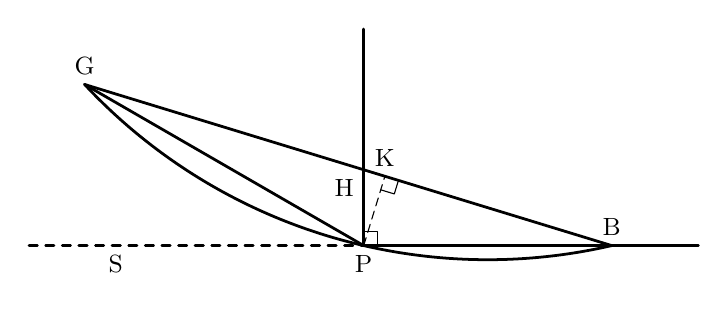
\begin{tikzpicture}[x=1cm,y=1cm, line cap=round, line join=round, font=\small]

% ============================================================
% A) THAM SỐ HÓA (chỉ chỉnh ở đây)
% ============================================================
\def\alpha{30}     % góc GPS (độ): giữa hai tia GP và PS
\def\LGB{7.0}      % độ dài dây cung GB (chọn tạm cho hài hòa)

% Bố cục (không ảnh hưởng bản chất hình học)
\def\bFrac{0.45}   % b = bFrac * R (phải < 2 để tâm O tồn tại). 1.2–1.6 thường đẹp.
\def\ExtLeft{4.25}  % kéo dài mặt đất về trái
\def\ExtRight{4.25} % kéo dài mặt đất về phải
\def\PHlen{2.75}    % độ dài tia PH

\def\PerpMark{0.18}% kích thước dấu vuông góc

% ============================================================
% B) TIỀN TÍNH HÌNH HỌC (ổn định, không intersections)
% ============================================================
% Góc giữa PG và PB là: angle GPB = 180 - alpha (vì PS là tia đối của PB)
% Dây GB có độ dài LGB => bán kính đường tròn ngoại tiếp:
%   LGB = 2 R sin(alpha)  =>  R = LGB / (2 sin alpha)
\pgfmathsetmacro{\R}{\LGB/(2*sin(\alpha))}

% Đặt P=(0,0), chọn B=(b,0) với b = bFrac*R, và tâm O=(b/2, h) sao cho |OP|=|OB|=R
\pgfmathsetmacro{\b}{\bFrac*\R}
% Điều kiện tồn tại tâm: b <= 2R  (tức bFrac <= 2)
\pgfmathsetmacro{\h}{sqrt(max(0,\R*\R-(\b/2)*(\b/2)))}
\pgfmathsetmacro{\Ox}{\b/2}
\pgfmathsetmacro{\Oy}{\h}

% Tia PS là trục âm Ox, tia GP tạo với PS góc alpha => hướng PG có góc phi = 180 - alpha
\pgfmathsetmacro{\phi}{180-\alpha}

% G là giao điểm khác P của tia PG với đường tròn (tâm O bán kính R)
% Ray: (x,y)=(t cos phi, t sin phi), t>=0.
% Solve: (x-Ox)^2 + (y-Oy)^2 = R^2  => t = 2*(Ox cos phi + Oy sin phi)
\pgfmathsetmacro{\tG}{2*(\Ox*cos(\phi)+\Oy*sin(\phi))}
\pgfmathsetmacro{\Gx}{\tG*cos(\phi)}
\pgfmathsetmacro{\Gy}{\tG*sin(\phi)}

% ============================================================
% C) ĐỊNH NGHĨA ĐIỂM
% ============================================================
\coordinate (P) at (0,0);
\coordinate (B) at (\b,0);
\coordinate (O) at (\Ox,\Oy);
\coordinate (G) at (\Gx,\Gy);

% Dây cung GB
% H = GB ∩ PH, mà PH là đường thẳng x=0
% GB: G + t(B-G),  tH=(0-Gx)/(Bx-Gx)
\pgfmathsetmacro{\vx}{\b-\Gx}
\pgfmathsetmacro{\vy}{0-\Gy}
\pgfmathsetmacro{\tH}{(0-\Gx)/(\b-\Gx)}
\pgfmathsetmacro{\Hx}{\Gx+\tH*\vx}
\pgfmathsetmacro{\Hy}{\Gy+\tH*\vy}
\coordinate (H) at (\Hx,\Hy);

% K = hình chiếu vuông góc của P lên đường thẳng GB (đảm bảo PK ⟂ GB)
% tK = ((P-G)·v)/(v·v)
\pgfmathsetmacro{\vv}{\vx*\vx+\vy*\vy}
\pgfmathsetmacro{\tK}{((0-\Gx)*\vx+(0-\Gy)*\vy)/\vv}
\pgfmathsetmacro{\Kx}{\Gx+\tK*\vx}
\pgfmathsetmacro{\Ky}{\Gy+\tK*\vy}
\coordinate (K) at (\Kx,\Ky);

% Góc tham số để vẽ cung tròn G->P và P->B trên cùng đường tròn (tâm O, bán kính R)
\pgfmathsetmacro{\angG}{atan2(\Gy-\Oy,\Gx-\Ox)}
\pgfmathsetmacro{\angP}{atan2(0-\Oy,0-\Ox)}
\pgfmathsetmacro{\angB}{atan2(0-\Oy,\b-\Ox)}
% Quy về [0,360) để arc ổn định
\pgfmathsetmacro{\angGpos}{ifthenelse(\angG<0,\angG+360,\angG)}
\pgfmathsetmacro{\angPpos}{ifthenelse(\angP<0,\angP+360,\angP)}
\pgfmathsetmacro{\angBpos}{ifthenelse(\angB<0,\angB+360,\angB)}

% ============================================================
% D) VẼ HÌNH (không khung)
% ============================================================

% 1) Mặt đất: PB là tia dương, PS là tia đối
\draw[dashed, line width=1.0pt] (-\ExtLeft,0) -- (P);
\draw[line width=1.0pt] (P) -- (\ExtRight,0);

% 2) Tia PH ⟂ PB (đường thẳng đứng qua P)
\draw[line width=1.0pt] (P) -- ($(P)+(0,\PHlen)$);

% 3) Tia PG (chỉ cần vẽ từ P qua G)
\draw[line width=1.0pt] (P) -- (G);

% 4) Dây cung GB
\draw[line width=1.0pt] (G) -- (B);

% 5) Cung tròn GPB (G, P, B cùng thuộc 1 đường tròn)
%    Vẽ hai cung: G->P và P->B để chắc chắn đi qua P.
\draw[line width=1.0pt] (G) arc[start angle=\angGpos, end angle=\angPpos, radius=\R];
\draw[line width=1.0pt] (P) arc[start angle=\angPpos, end angle=\angBpos, radius=\R];

% 6) PK ⟂ GB (nét đứt như hình)
\draw[densely dashed] (P) -- (K);

% 7) (tùy chọn) dấu vuông góc tại P (PH ⟂ PB)
\draw (P) -- ++(\PerpMark,0) -- ++(0,\PerpMark) -- ++(-\PerpMark,0);

% 8) (tùy chọn) dấu vuông góc tại K (PK ⟂ GB)
%    Hướng đơn vị theo GB và theo KP để vẽ ô góc vuông
\pgfmathsetmacro{\Lv}{sqrt(\vv)}
\pgfmathsetmacro{\ux}{\vx/\Lv}
\pgfmathsetmacro{\uy}{\vy/\Lv}
\pgfmathsetmacro{\kpx}{0-\Kx}
\pgfmathsetmacro{\kpy}{0-\Ky}
\pgfmathsetmacro{\Lkp}{sqrt(\kpx*\kpx+\kpy*\kpy)}
\pgfmathsetmacro{\px}{\kpx/\Lkp}
\pgfmathsetmacro{\py}{\kpy/\Lkp}
\coordinate (K1) at ($(K)+\PerpMark*(\ux,\uy)$);
\coordinate (K2) at ($(K)+\PerpMark*(\px,\py)$);
\coordinate (K3) at ($(K1)+\PerpMark*(\px,\py)$);
\draw (K) -- (K1) -- (K3) -- (K2);

% ============================================================
% E) NHÃN (có thể bỏ/đổi vị trí tùy bạn)
% ============================================================
\node[above]        at (G) {G};
\node[below left]  at (H) {H};
\node[above] at (K) {K};
\node[below]       at (P) {P};
\node[above] at (B) {B};
\node[below] at ($(P)-(B)$) {S};

\end{tikzpicture}
\end{document}
